\chapter{Bootstrapping Blockchains}
\section{Introduction}
Today, the security of established blockchains like Bitcoin and Ethereum is often taken for granted. This confidence is based on several factors, including the historical track record of these blockchains, which have not experienced any fatal attacks thus far. Additionally, mathematical models provide provable guarantees that demonstrate the difficulty an adversary would face in attempting to attack the system. For instance, it's established that an attacker must control nearly 50\% of the mining power in the system to mount an effective attack. \\
In the case of Bitcoin, the total mining power has reached a level where it can compute over $10^{20}$ hashes per second, a staggering number compared to the hash rate of a modern GPU, which is around $10^{8}$ hashes per second. This immense computing power makes it economically unfeasible for an adversary to amass such resources. In essence, Bitcoin's security is rooted in the substantial computing power that has been invested into the network.\\
However, during its early days, Bitcoin didn't enjoy such a high level of security. With a much smaller number of miners participating, the hash rate was closer to $10^{6}$ hashes per second. At that time, matching this hash rate would have been relatively easier for an adversary, even using the computing resources available in 2009. This highlights the security challenge faced by new blockchains that start with a significantly lower total computational power compared to well-established networks like Bitcoin and Ethereum.\\
This lecture aims to address the issue of "bootstrapping" security for new blockchains, focusing initially on both Proof-of-Work (PoW) and Proof-of-Stake (PoS) systems. The goal is to ensure that these emerging blockchains can establish a strong security foundation despite their lower initial computational power. Various methods, including techniques for PoW and PoS systems, will be explored. Additionally, the lecture will discuss strategies for leveraging the security of existing blockchains, known as "piggybacking," to enhance the security of new blockchain networks.
\section{Bootstrapping PoW Blockchains}
Bootstrapping Proof of Work (PoW) blockchains involves employing various principles to establish their security and functionality. These principles are not mutually exclusive and can be combined to create a robust and secure PoW blockchain system. Here are some key principles:
\begin{enumerate}
	\item \textbf{Incentives}
	\item \textbf{Checkpointing}
	\item \textbf{Hardfork}
	\item \textbf{Proof of Burn}
	\item \textbf{Softfork}
\end{enumerate}
By applying these principles or a combination of them, PoW blockchains can bootstrap their security and functionality. Each principle addresses different aspects of network security, participant incentives, and protocol upgrades. As the blockchain ecosystem evolves, these principles may be adapted and refined to suit the specific needs of new PoW blockchains.
\subsection{Incentives}
The security of Proof of Work (PoW) blockchains is often rooted in the rational behavior of miners, who are economically motivated to act in the best interest of the system. This incentive-based security measure relies on miners' rationality and their economic self-interest to maintain the integrity of the blockchain.\\
In a well-designed incentive-compatible blockchain system, it is improbable that a coalition of miners controlling a majority of the mining power would collaborate to attack the network. This is because such an attack would be counterproductive and economically detrimental to the miners themselves. While this approach does not guarantee security against a 51\% attack, it provides a strong deterrent against malicious behavior.\\
In the steady-state operation of a PoW blockchain, mining rewards play a significant role in incentivizing miners to behave honestly. This incentive extends to the early stages of the blockchain's existence. To further encourage honest behavior, some PoW blockchains implement a mechanism that provides extra incentives to early miners. For example, Bitcoin initially offered a mining reward of $50$ bitcoins per mined block, which decreased over time through a programmed halving process.\\
While the initial block rewards were of limited monetary value, early miners were driven by the anticipation that the value of Bitcoin would increase with wider adoption. This belief proved accurate as Bitcoin gained popularity, see Figure \ref{fig:L18_f1}. Miners with substantial mining power recognized that maintaining the security and reputation of the blockchain through honest participation would lead to significant future gains. On the other hand, engaging in malicious activities, such as double-spending attacks, might yield short-term gains but would ultimately devalue the cryptocurrency.\\
\begin{center}
	\begin{figure}
		\centering
		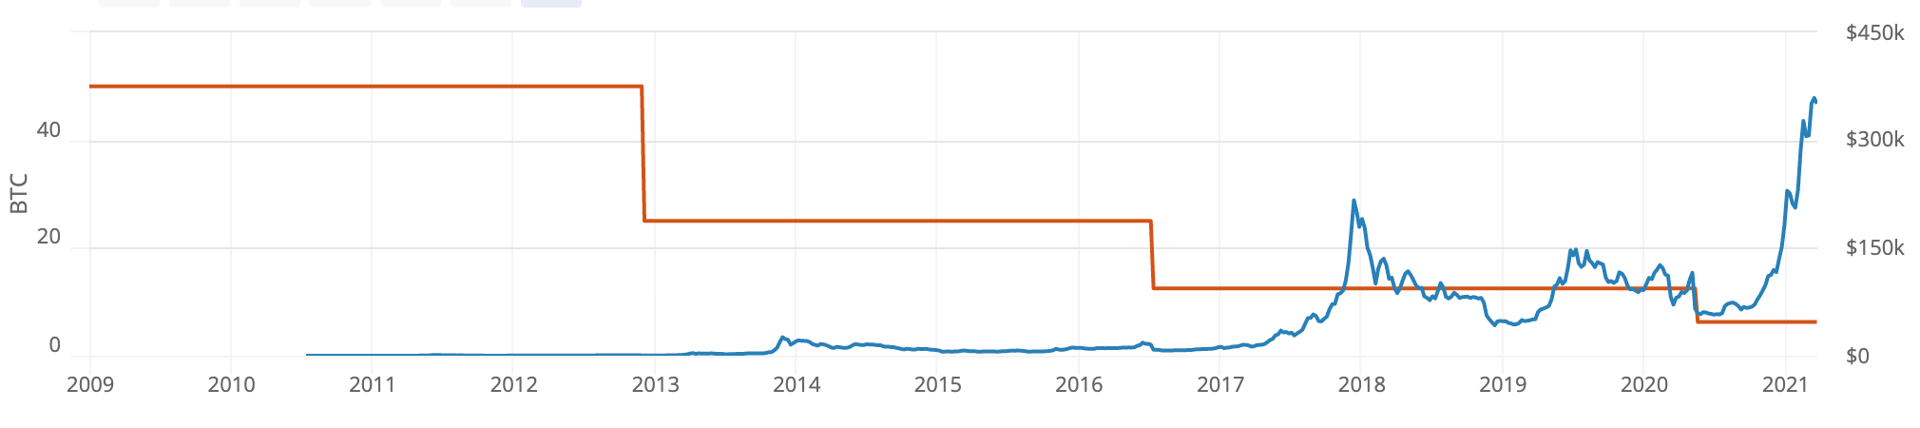
\includegraphics[width=0.8\linewidth]{Fig/18/F1}
		\caption{Block rewards value in Bitcoin and dollar over time}
		\label{fig:L18_f1}
	\end{figure}
\end{center}
In essence, the correct incentives aligned with miners' economic interests and played a pivotal role in ensuring the security of PoW blockchains, particularly during their early stages. By creating economic disincentives for malicious behavior and fostering a long-term view of value preservation, incentive-based security measures have contributed to the overall stability and trustworthiness of PoW-based cryptocurrencies like Bitcoin.
\subsection{Checkpointing}
A secondary approach to initiating Proof of Work (PoW) blockchains involves the implementation of a checkpointing mechanism. In a broad sense, this technique relies on a trusted entity, or a consortium of entities (see Figure \ref{fig:L18_f2}), to periodically establish checkpoints for blocks. New blocks are then required to be mined beneath the latest checkpoint to attain validation. Users can leverage these checkpoints for confirmation, essentially validating blocks up to the most recent checkpoint. This checkpointing process essentially functions as a Byzantine Fault Tolerant (BFT) consensus protocol, orchestrated by a specialized group known as checkpointers.\\
In a prior lecture, we learned about the role of checkpointing, often facilitated through a finality gadget, in enhancing the security of the longest-chain protocol during periods of asynchrony. Similarly, the checkpointing mechanism can act as a safeguard against an adversary wielding over 50\% of mining power, provided the checkpointing process operates reliably. Notably, it is crucial to recognize that the selection of checkpointers is not governed by the traditional mining process. Instead, these checkpointers consist of reputable entities, such as corporations or foundations, chosen with the primary goal of securing the PoW blockchain's early stages. Consequently, there's a reasonable assumption that a majority or super-majority of checkpointers will uphold honesty.\\
\begin{center}
	\begin{figure}
		\centering
		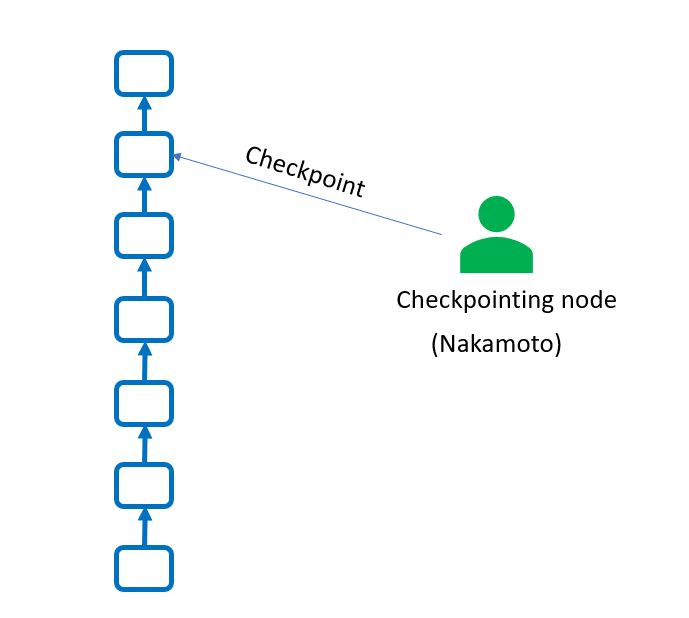
\includegraphics[width=0.5\linewidth]{Fig/18/F2}
		\caption{Checkpointing is a method of bootstrapping PoW blockchains that employs a trusted party (or a group of parties) that checkpoints blocks at regular intervals.}
		\label{fig:L18_f2}
	\end{figure}
\end{center}
Examining the security of such a checkpointing-based protocol in the presence of an adversary with majority mining power reveals that safety is readily arguable, as it hinges on the underlying checkpointing mechanism's safety properties. However, ensuring liveness can pose a more intricate challenge. A simplistic implementation of checkpointing may yield subpar liveness guarantees, as illustrated in Figure \ref{fig:L18_f4}.
\begin{center}
	\begin{figure}
		\centering
		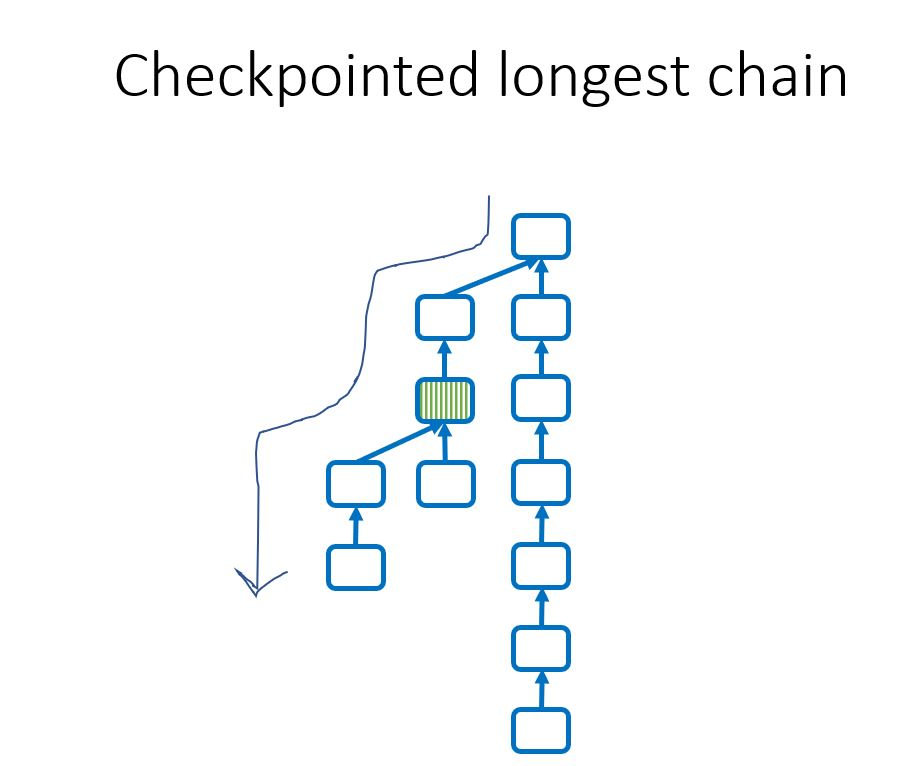
\includegraphics[width=0.5\linewidth]{Fig/18/F3}
		\caption{A checkpointed longest chain is a blockchain that employs checkpoints to ensure that new blocks are mined below the latest checkpoint to be considered valid.}
		\label{fig:f3}
	\end{figure}
\end{center}
Liveness is of paramount importance to incentivize honest nodes to remain active within the system, see Figure \ref{fig:L18_f5}. In the absence of honest blocks being included in the ledger, honest miners would be unable to accumulate rewards, potentially leading them to exit the system. While earlier checkpoint-based protocols may have been willing to compromise liveness during periods of asynchrony, the situation changes when an adversary maintains a mining majority for an extended period, potentially deterring new user adoption.\\
Two fundamental principles are pivotal in establishing a checkpointing mechanism that guarantees liveness in the face of an adversary with more than 50\% mining power:
\begin{center}
	\begin{figure}
		\centering
		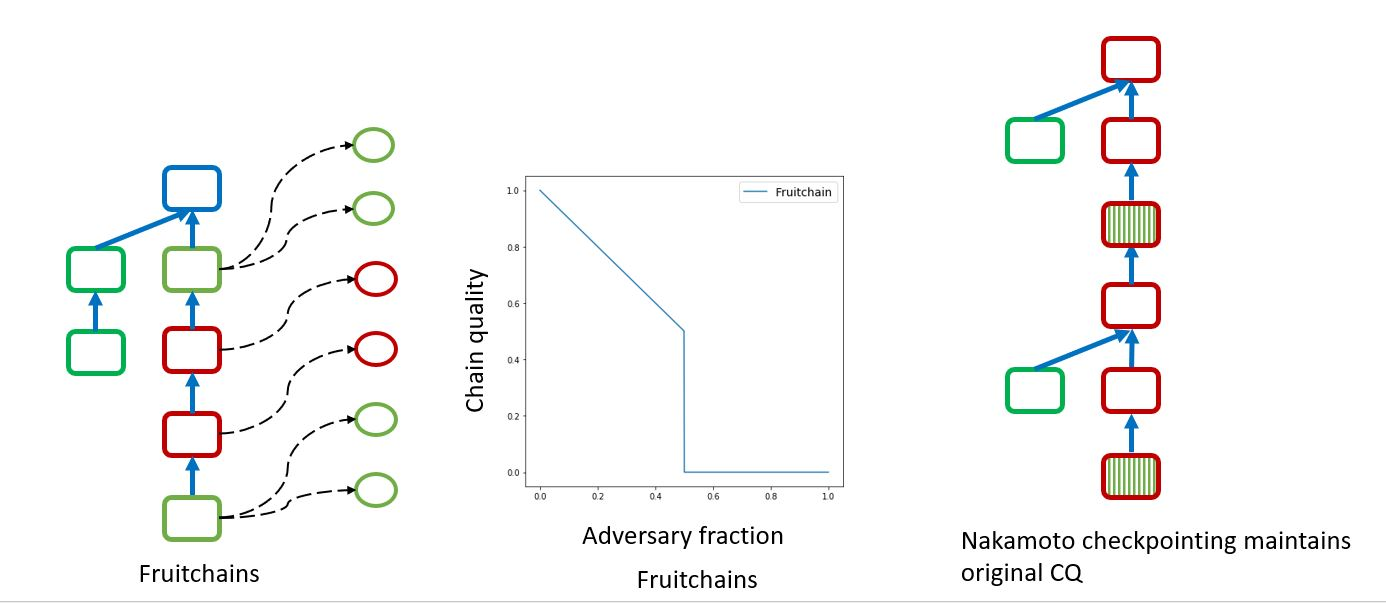
\includegraphics[width=0.8\linewidth]{Fig/18/F4}
		\caption{(a) The green and blue blocks are called “fruitchains”, which are subchains that are generated by honest nodes but do not have enough proof-of-work to be part of the main chain. (b) The graph shows that the chain quality drops to zero when the adversary fraction reaches 0.5, meaning that the blockchain becomes completely controlled by malicious nodes. (c) How checkpointing can help maintain the original chain quality, even when the adversary fraction is greater than 0.5. The red blocks are called “Nakamoto checkpoints”, which are blocks that have enough proof-of-work to be accepted by the network as valid checkpoints.}
		\label{fig:L18_f4}
	\end{figure}
\end{center}
\begin{enumerate}
	\item \textbf{Fresh Random String with Every Checkpoint:} Checkpointers should generate a new, unique random string with each checkpoint. This random string must be incorporated into all descendant blocks of the checkpoint. This approach ensures that blocks following a checkpoint are mined subsequent to the checkpoint's establishment. By resetting the block counter with every checkpoint block, the adversary's ability to exploit mining power by preemptively generating numerous blocks is curtailed.
	\item \textbf{Introducing Reference Links to Honest Blocks:} Checkpoints should incorporate reference links to blocks not on the main chain but likely to be honest. This concept stems from the fact that honest blocks are produced in proportion to honest mining power, although they might not always find their place on the main chain due to adversarial interference. These reference links serve to bring these honest blocks into the ledger, enhancing chain quality to align with honest mining power. This approach, exemplified by FruitChains, bolsters the overall system's resilience and security.
\end{enumerate}
\begin{figure}[h!]
	\centering
	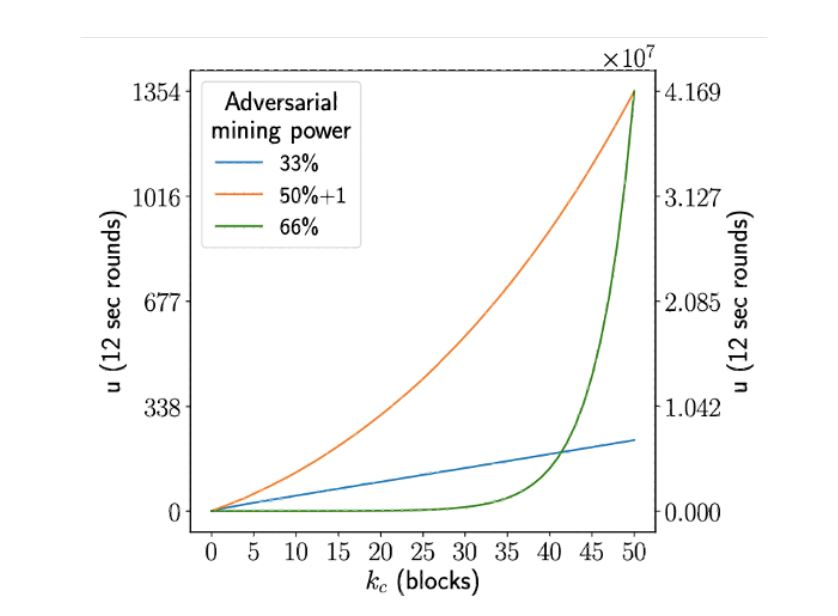
\includegraphics[width=0.8\linewidth]{Fig/18/F5}
	\caption{Chain Quality degrades sharply with an increase in the adversarial mining power, and	with an increase in the epoch length (period between checkpoints)}
	\label{fig:L18_f5}
\end{figure}
These principles, collectively illustrated in Figure \ref{fig:L18_f6}, contribute to the establishment of a robust checkpointing mechanism that ensures both safety and liveness under the presence of a dominant adversary. Notably, historical practices within Bitcoin involved checkpoint issuance at regular intervals by Satoshi Nakamoto. However, this practice was discontinued in 2014, likely due to Bitcoin's growing mining power rendering it self-sufficient. A more resilient approach would involve a permissioned set of users engaged in the checkpointing process.\\
\begin{center}
	\begin{figure}
		\centering
		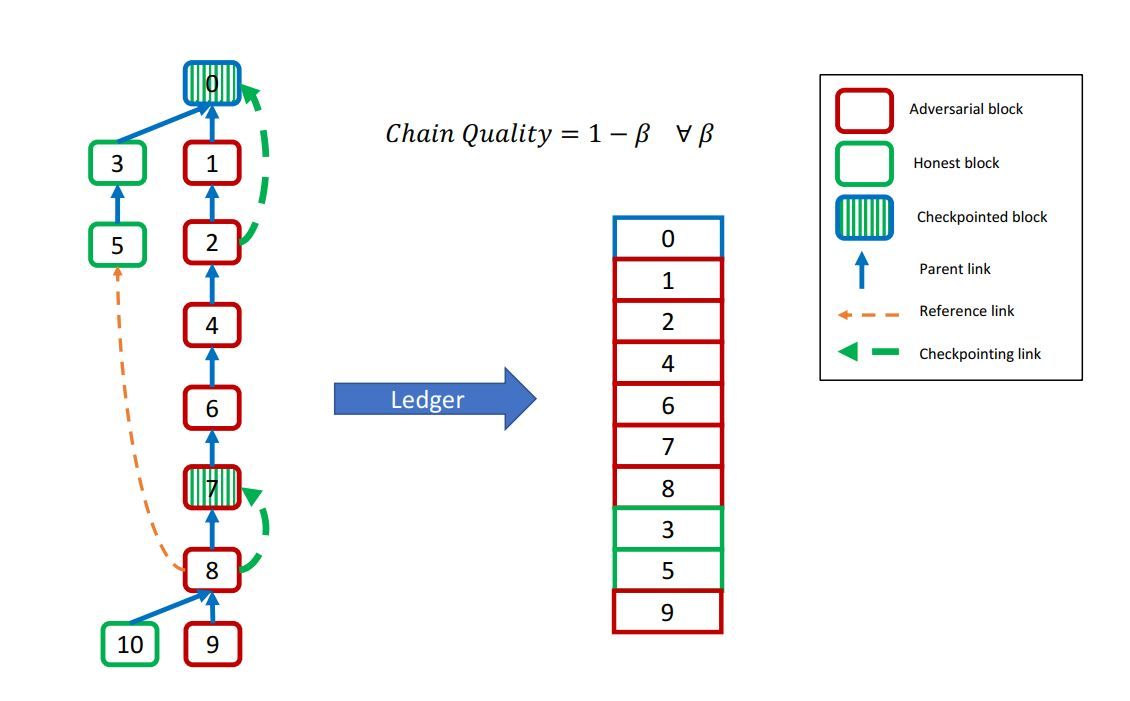
\includegraphics[width=0.8\linewidth]{Fig/18/F6}
		\caption{The Advocate system, which provides optimal chain quality even in the presence of an adversarial majority. Such a system provides a useful checkpointing mechanism to bootstrap PoW blockchains}
		\label{fig:L18_f6}
	\end{figure}
\end{center}
\textbf{Ledger sanitization}, which is a process of removing unnecessary or redundant information from a ledger. A ledger is a record of transactions that are verified and stored by a network of nodes. Ledger sanitization can help improve the efficiency and security of the ledger, as well as protect the privacy of the users, see Figure \ref{fig:L18_f7}.
\begin{figure}[h!]
	\centering
	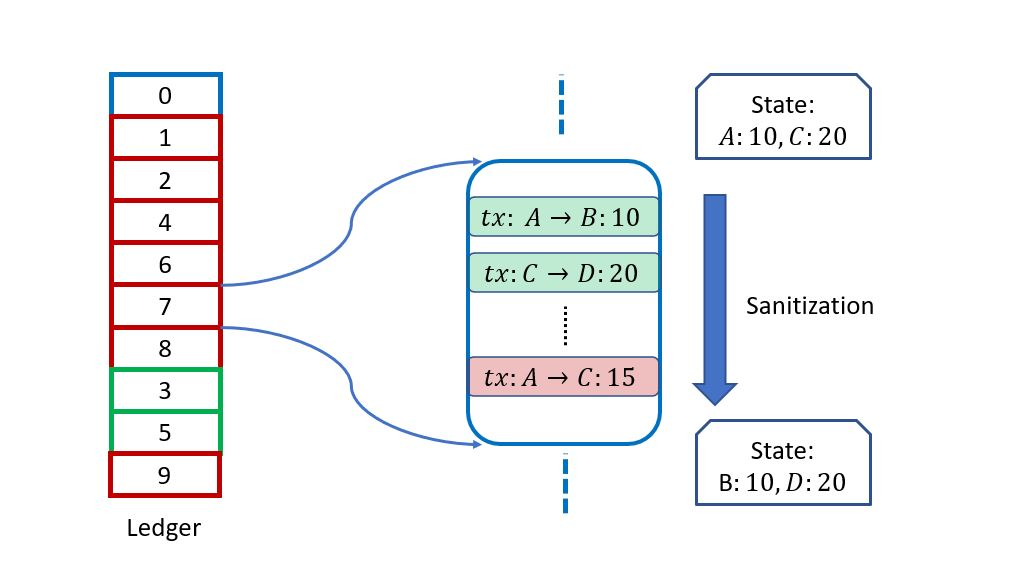
\includegraphics[width=0.8\linewidth]{Fig/18/F7}
	\caption{The diagram shows how the ledger can be simplified by removing some numbers that are not relevant to the current state of the ledger.}
	\label{fig:L18_f7}
\end{figure}
\textbf{BFT-SMR} is a technique that ensures that the nodes agree on the same state of the system, even if some of them are malicious or faulty. Checkpointing is a technique that prevents an attacker from rewriting the history of the blockchain by creating a longer chain with more proof-of-work. The Figure \ref{fig:L18_f8} illustrates how Advocate uses two chains: a main chain and a checkpoint chain, and how the nodes communicate with each other using different types of links, such as proven links, witness links, and checkpointing links. This Figure also shows how Advocate can recover from a fault scenario, where a malicious node tries to create a fork in the main chain, by switching to a different leader node and extending from the last checkpoint.
\begin{figure}[h!]
	\centering
	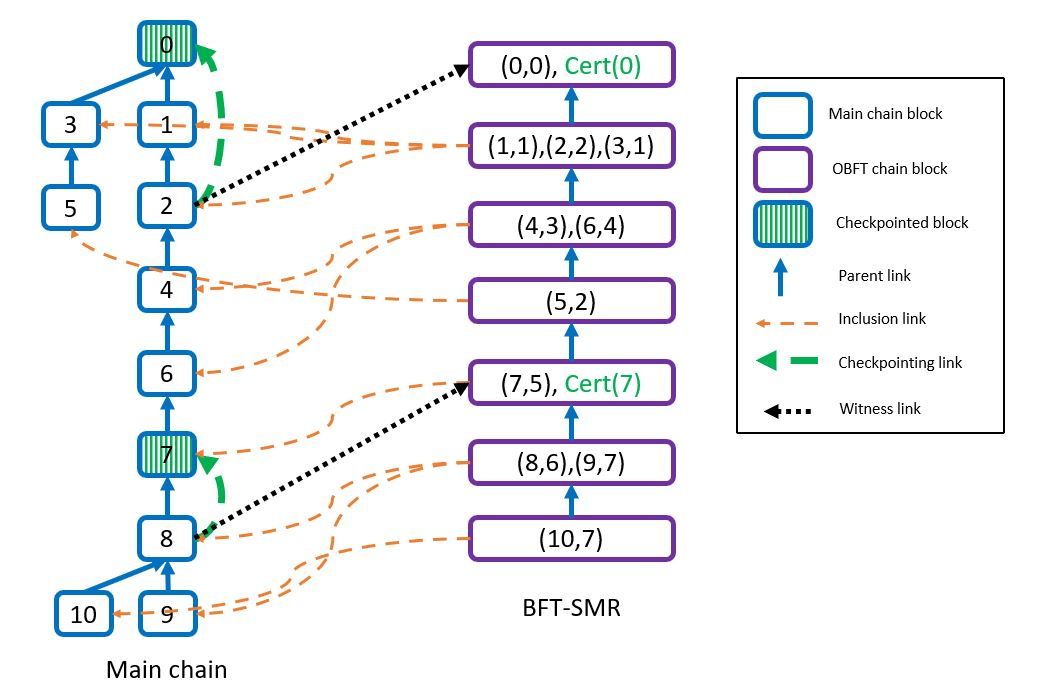
\includegraphics[width=0.8\linewidth]{Fig/18/F8}
	\caption{This image shows how a blockchain system called Advocate uses BFT-SMR and checkpointing to achieve consensus among the nodes in the network.}
	\label{fig:L18_f8}
\end{figure}

\noindent \textbf{Advocate using external chains.} Advocate uses Bitcoin as an external chain to achieve consensus among the nodes in the network. Consensus is the process of ensuring that the nodes agree on the same state of the system, even if some of them are malicious or faulty. The Figure \ref{fig:L18_f9} shows how Advocate uses two chains: a main chain and a federation, and how they communicate with each other using different types of links, such as checkpointing links, witness links, and reference links. The picture also shows how Advocate uses availability voting and checkpointing to prevent forks and secure the main chain.
\begin{figure}[h!]
	\centering
	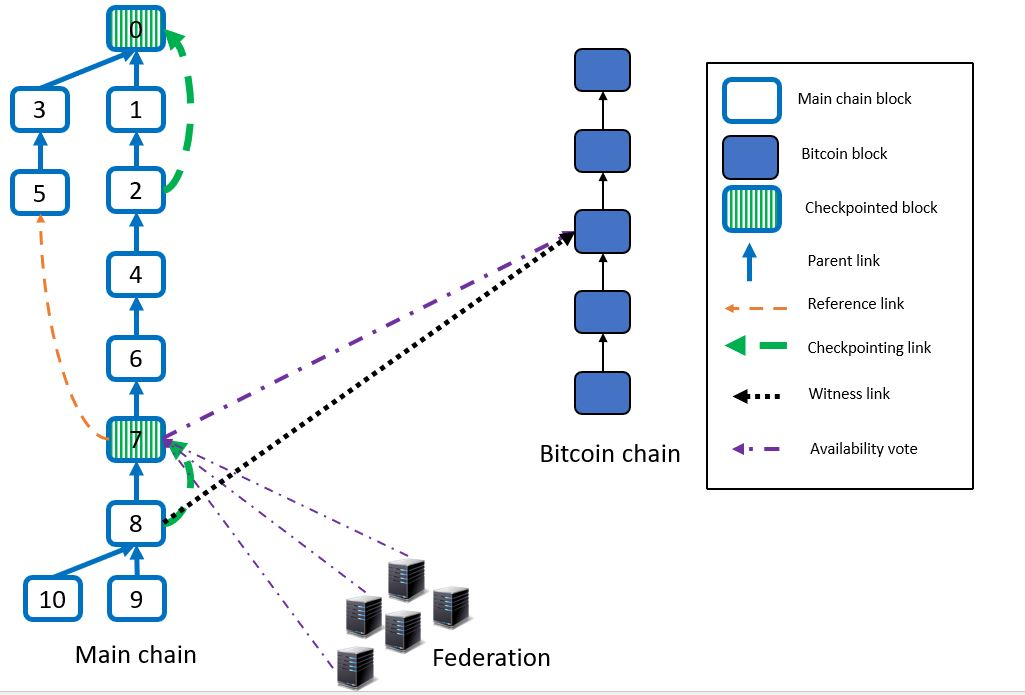
\includegraphics[width=0.8\linewidth]{Fig/18/F9}
	\caption{How to advocate using external chains. External chains are blockchains that are not part of the main chain, but can be used to provide additional security and functionality for the main chain.}
	\label{fig:L18_f9}
\end{figure}
\subsection{Hardfork}
In the realm of blockchain technology, a \textit{hard fork}(or hardfork) signifies a pivotal juncture in the blockchain's protocol where substantial changes are introduced, rendering them incompatible with the previous version. Blocks generated under the new protocol are considered invalid according to the old protocol, and vice versa. Hardforks can serve various purposes, such as integrating new features to enhance security or performance, as well as rectifying security vulnerabilities within the existing codebase – as was the case with Ethereum's response to the \href{https://en.wikipedia.org/wiki/The_DAO_(organization)}{DAO vulnerability}.\\
To grasp the concept of hardforks better, consider the following scenario. Imagine that the Bitcoin miners collectively decide to amplify Bitcoin's mining rate by a factor of ten in order to boost its transaction throughput. Achieving this would necessitate a reduction in block difficulty. While a simultaneous, unanimous agreement on this alteration is impractical in a decentralized system, as some nodes might remain unaware of the changes temporarily, creating a split. Nodes uninformed of the new rules will disregard blocks generated under the updated protocol, deeming them invalid. This situation gives rise to a significant divergence in the blockchain's development – the phenomenon known as a hardfork.\\
In certain instances, eventually, all nodes converge on adopting the software update. In such cases, the fork aligned with the older block format ceases to progress, while the one following the new format continues its growth. Conversely, there are scenarios where a subset of nodes embraces the update while others remain resistant. This results in two divergent forks coexisting indefinitely. Essentially, the fork adhering to the updated protocol forms a new cryptocurrency or blockchain system. The occurrence of a hardfork signifies the inception of this fresh system. Some nodes migrate to this new setup, while others persist within the original one. Importantly, this phenomenon isn't a security vulnerability; once a node unequivocally selects which version of the software to follow, the blockchain ensures its security.\\
Numerous cryptocurrencies have been launched through hardforks, with Bitcoin Cash – a hardfork from Bitcoin – standing as a notable example (The history of hard forks from Bitcoin can be found \href{https://www.investopedia.com/tech/history-bitcoin-hard-forks/}{here}.). When a new cryptocurrency originates from an established blockchain through a hardfork, it inherits the coin distribution (or more broadly, the system's state) recorded in the final block prior to the fork. If the new system proves appealing, it can rapidly amass a substantial number of miners (representing significant computational power) due to seamless migration from the old system. This imparts robust security to the new system from the outset, establishing a strong decentralized foundation. Furthermore, the new system inherits most of the security attributes from the pre-existing blockchain, necessitating verification solely for the new features introduced.
\subsection{Soft Forks}
Soft forks, in contrast to hard forks, represent software updates that maintain backward compatibility. Under a soft fork, even individuals who haven't yet upgraded their software will consider new blocks valid. It's conceivable that those adopting the new update could regard old blocks as invalid. Nonetheless, if a majority of miners embrace the updated software, the blockchain can operate seamlessly. Blocks produced using the old software will swiftly become outdated. Soft forks provide a gradual transition to a new system compared to the more abrupt approach of hard forks. However, for a soft fork to take effect, a majority of miners must be utilizing the updated software. Similar to hard forks, soft forks serve as a means to introduce improved features to an existing system.\\
Within the context of Bitcoin, soft forks have been employed to introduce new transaction types or scripts. A notable instance of this is the Segregated Witness (SegWit) update. As a reminder, Bitcoin blocks possess a maximum size of 1MB, placing a constraint on the number of transactions that can be accommodated within a block. SegWit is a proposal aimed at reducing the size of Bitcoin transactions, thereby enabling a higher transaction throughput while still adhering to the 1MB block size limit.\\
The fundamental concept behind SegWit involves segregating transaction signatures from the main block. Every Bitcoin transaction necessitates a signature, which can occupy up to 65\% of the transaction's space. By separating the signature, the transaction size is reduced. Importantly, the signatures remain intact; they are merely relocated to an additional segment of the block that doesn't contribute to the 1MB limit. The term "segregated witness" accurately captures this design principle, with "witness" referring to the transaction signatures that are partitioned from the main block.
\subsection{Proof of Burn}
Proof of burn is a strategy through which users can transition from an existing blockchain system, such as Bitcoin, to a novel one. This process involves "burning" coins, whereby nodes send Bitcoins to an address that is verifiably unspendable. This unspendable address typically possesses a fixed public key for which deriving the corresponding secret key is virtually impossible. In return for burning these coins, users receive rewards denominated in the native currency of the new blockchain. Additionally, users might obtain mining privileges proportionate to the quantity of coins they have burned. This mechanism effectively establishes a fresh system wherein mining power correlates with the amount of funds that have been burned.\\
In comparison to the resource-intensive Proof-of-Work approach, the proof-of-burn method is less demanding on resources while maintaining an equivalent level of security. It leverages the foundation of an established blockchain to facilitate this transition. Further details on this concept can be explored through this \href{https://en.bitcoin.it/wiki/Proof_of_burn}{source}.
\section{Bootstrapping PoS Blockchains}
In a Proof of Stake (PoS) system, the selection of block proposers is based on the stake or coins that nodes hold and have recorded in the blockchain ledger. For a PoS system to initiate, an initial amount of stake (coins) must be distributed among the initial participants. This initial stake distribution is noted in the genesis block, which is the first block of the blockchain. Unlike Proof of Work (PoW) blockchains like Bitcoin, where the genesis block doesn't necessarily record ownership of coins, PoS systems require an initial stake distribution to function properly.\\
However, PoS systems can potentially suffer from a "rich-get-richer" phenomenon. This means that participants with higher stakes are more likely to be selected as block proposers and, consequently, receive block and transaction rewards. This increased reward accumulation enhances their likelihood of mining future blocks as well, potentially leading to centralization of control.\\
There are strategies to mitigate this issue and promote a more balanced distribution of stake:
\begin{enumerate}
	\item \textbf{Uniform Initial Stake Distribution:} Starting with a relatively large and uniformly distributed initial stake across nodes can reduce the impact of the rich-get-richer effect. This means that the initial stake is substantial in relation to the rewards earned from blocks and transactions.
	\item \textbf{Dynamic Reward Design:} Designing the mining rewards to increase over time can also help. When rewards increase, the stake distribution over time is more likely to become more uniform compared to scenarios where rewards remain constant or decrease.
\end{enumerate}
Several methods can be employed to establish the initial set of stakeholders in a PoS-based cryptocurrency:
\begin{enumerate}
	\item \textbf{Proof-of-Burn Strategy:} This involves requiring users to "burn" or lock up coins from an existing system in exchange for new coins in the new PoS-based system.
	\item \textbf{Airdrops:} Distributing a small amount of coins for free to a wide range of users helps create an initial user base. Airdrops could be given for performing certain actions, like tweeting about the new currency, which also increases visibility and popularity.
	\item \textbf{Initial Coin Offering (ICO):} Similar to an Initial Public Offering (IPO), an ICO involves offering new tokens for sale at a fixed price in a fiat currency (e.g., dollars). ICOs are used as investment opportunities by users, although they also carry inherent risks.
\end{enumerate}
It's worth noting that these strategies can also be used in PoW-based blockchains to establish an initial user base and encourage participation. However, they become particularly crucial in PoS-based blockchains to ensure the necessary distribution of stake and participation to initiate the system and prevent centralization tendencies.
\section{Bootstrapping via Layer 2 Solutions}
In the present landscape, numerous new tokens are introduced on the Ethereum Virtual Machine Platform. This platform boasts remarkable flexibility and accommodates a diverse array of functionalities. These tokens capitalize on the inherent security of the Ethereum ledger, which is underpinned by Nakamoto consensus, and are meticulously designed to cater to specific applications. Essentially, each new token functions as an autonomous cryptocurrency, serving a distinct purpose (for instance, exclusive use within Walmart's ecosystem). By harnessing the foundation of Ethereum, these tokens inherit fundamental safety features without incurring additional effort.\\
A significant portion of tokens within the Ethereum ecosystem adhere to the "ERC-20" standard. This standard delineates essential guidelines, encompassing facets like token transfers, generation of new tokens, and more. The establishment of a standardized framework ensures seamless compatibility and facilitates effortless interchangeability among these tokens. Furthermore, ERC-20 tokens are harmonious with the overarching Ethereum infrastructure. Notably, all gas fees for transactions involving ERC-20 tokens are denominated in ETH, Ethereum's native cryptocurrency.\\
Once a token is integrated into the Ethereum ecosystem, innovative methods can be employed to encourage widespread adoption, leveraging the capabilities of smart contracts. A notable example is the employment of bonding curve contracts, which dynamically adjust the token's price in relation to its demand, often denominated in ETH or another currency. As demand surges, the token's price ascends, offering preferential rates to early adopters. This incentivizes early participation and fosters organic growth.\\
Smart contracts can also automate Initial Coin Offerings (ICOs), a fundraising mechanism common in the cryptocurrency space. Through these automated contracts, the issuance and distribution of new tokens can be orchestrated seamlessly, streamlining the process and enhancing accessibility for potential investors.\\
In essence, Ethereum's versatility and smart contract capabilities provide a fertile ground for the creation and deployment of novel tokens, each tailored to serve unique purposes while harnessing the collective security and infrastructure of the Ethereum platform.